% !TEX root = ../thesis_main.tex



\clearpage	
\chapter{Results}
\label{results_chapter}

\section{Measured Limits on $b_{Fierz}$, $C_S$, $C_T$}
	%\\*
	Results go here, with measured limits described and quantified in all formats anyone could ever care about.
	
\begin{figure}[h!!!t]
	\centering
	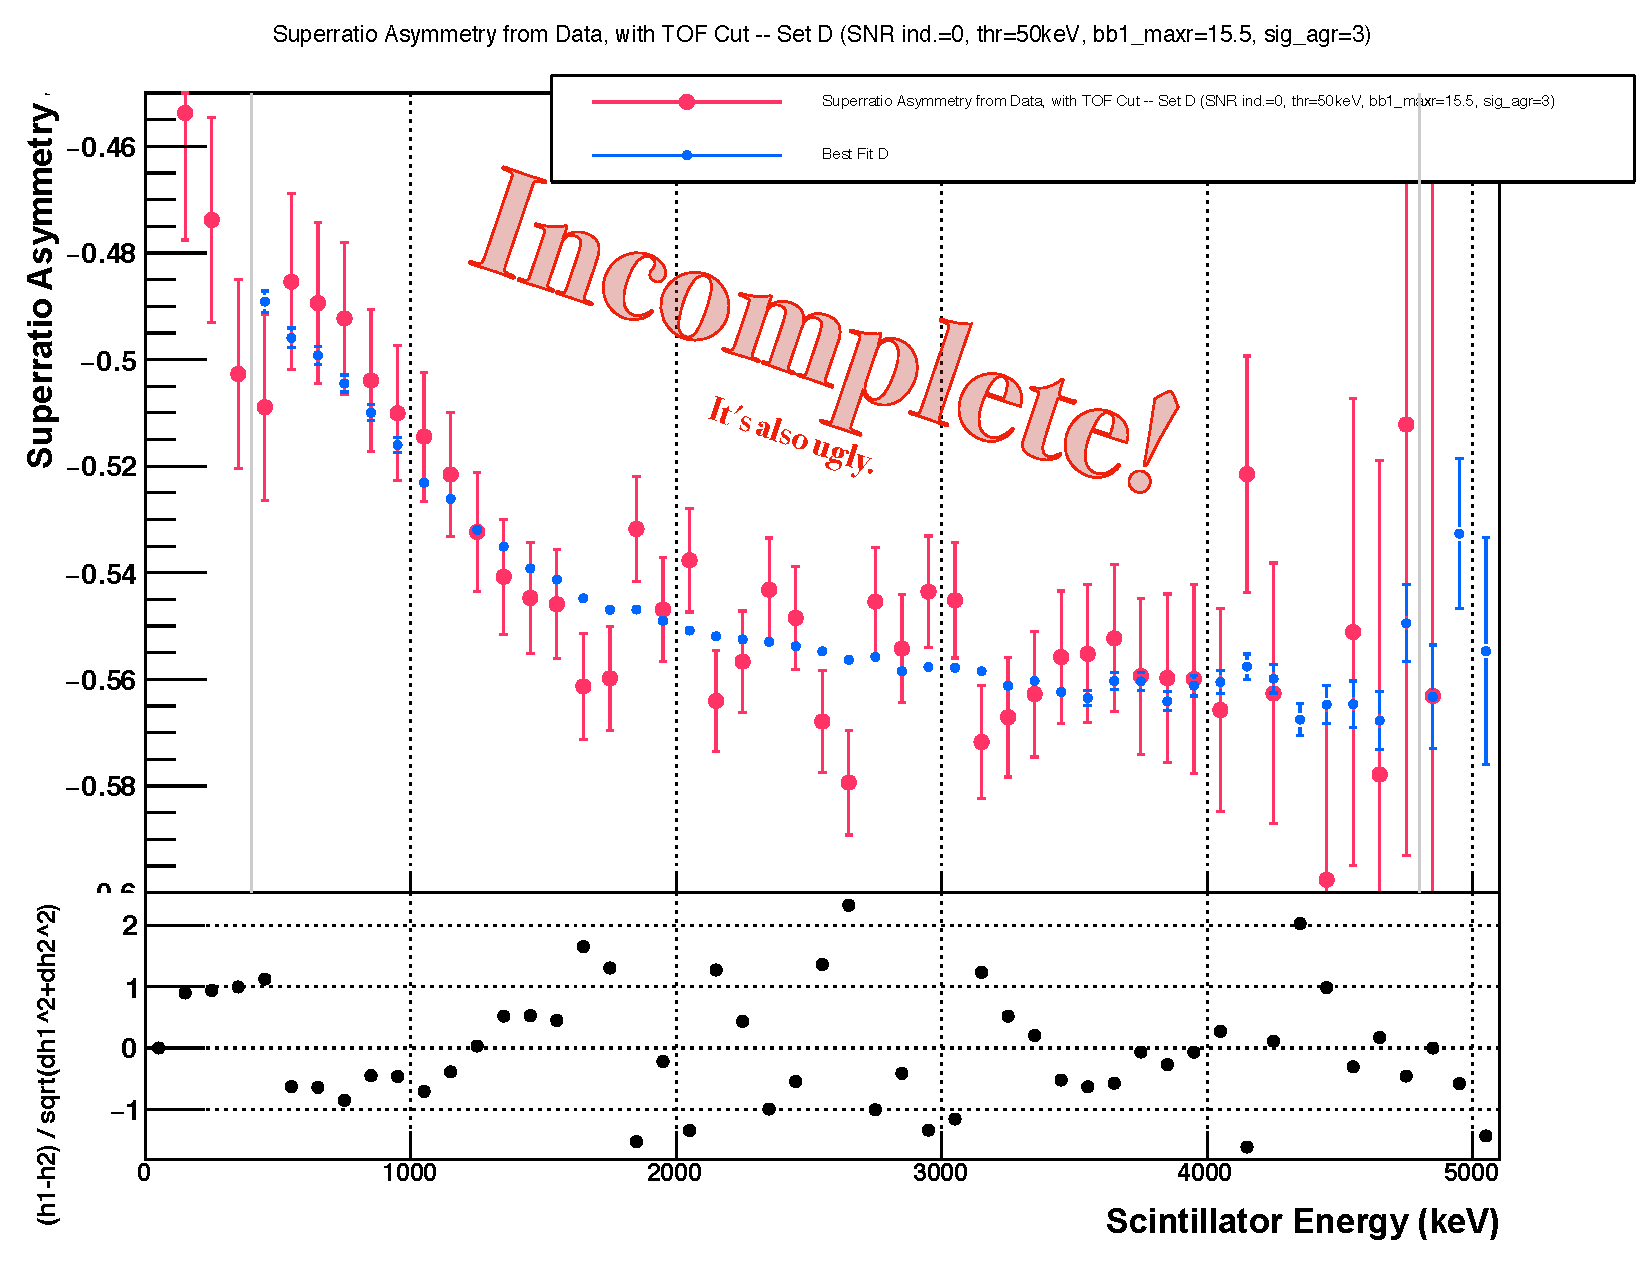
\includegraphics[width=.999\linewidth]
	{Figures/AsymmetryAndResiduals.pdf}
	\caption{A superratio asymmetry from the data, and the best fit from simulations.}	
	\label{fig:asymmetry}
\end{figure}
	
	
\begin{figure}[h!!!t]
	\centering
	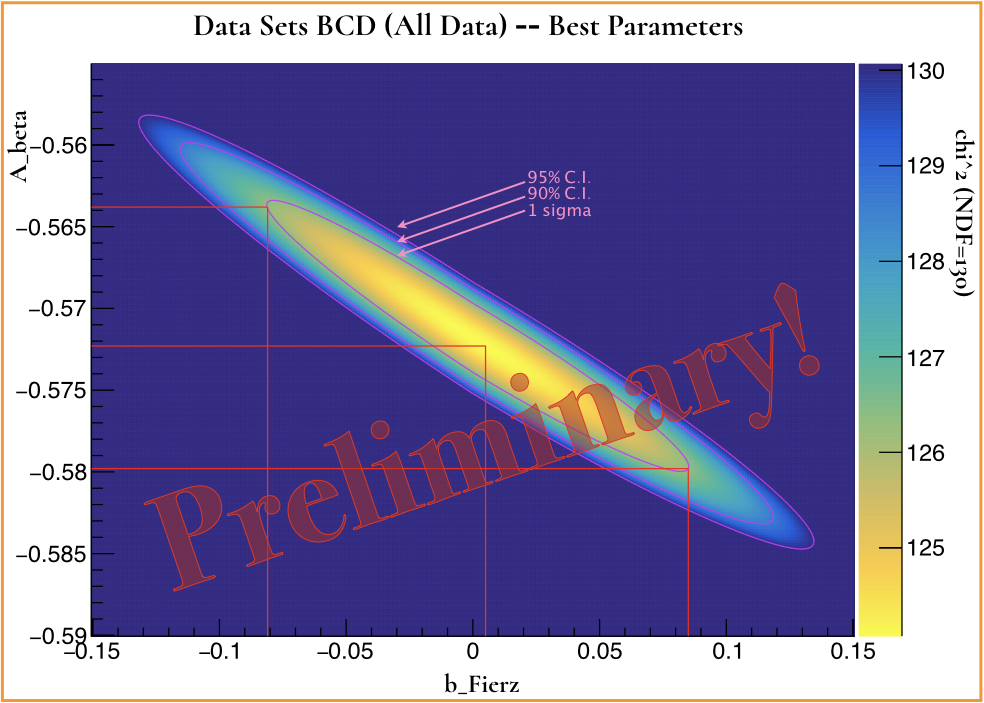
\includegraphics[width=.999\linewidth]
	{Figures/Abeta_bFierz_2D_prelim.png}
	\caption{Some results.  I'll want to show at least one of these things.  Probably show a separate one for each runset, actually.}	
	\label{fig:2d_results_bcd}
\end{figure}

\section{Discussion of Corrections and Uncertainties}
	...
	
\section{Relation to Other Measurements and New Overall Limits}
	%\\*
	In which I'll show exclusion plots and write down new limits, combining my result with results from the literature.


\section{Conclusions and Future Work}
